\section{Die Extraktion Produktspezifischer Daten}
\label{sec:extraktion-produktspezifischer-daten}

Der Parser ist dafür verantwortlich die für den Vergleich relevanten Produktinformationen aus HTML-Dateien zu
extrahieren und zu normalisieren.
Dies sind wichtige Prozessschritte, da die Qualität der extrahierten Werte die Ergebnisse der Matcher-Komponente
stark beeinflussen.

\subsection{Die technischen Anforderungen an den Parser}
\label{subsec:technische-anforderungen-parser}

Die Herausforderung der Parser-Komponente besteht hauptsächlich darin, das heterogene Informationsschemata der
verschiedenen Shops in ein homogenes, genormtes Schema zu bringen.

Im Detail geht es darum, zu jedem Angebot den Titel, die Produktbeschreibung, den Preis, die Marke, die Kategorie,
die Produktbilder sowie weitere eindeutige Merkmale im Format von idealo zu erfassen.
Diese eindeutigen Merkmale sind zum Beispiel die standardisierte EAN (Europäische Artikelnummer), HAN (Händler
Artikelnummer) und SKU (Stock keeping unit -- eine Shop-spezifische Kennung).

Da die Crawler-Komponente viel Zeit benötigt um alle Seiten zu erfassen, spielt die Laufzeit des Parsers eine
untergeordnete Rolle.
Eine schnelle Verarbeitung der Seiten ist dennoch wünschenswert, um eine gute Skalierbarkeit zu gewährleisten.

Es gilt sowohl eine hohe Trefferzahl als auch eine hohe Genauigkeit zu erzielen, damit die  Ergebnisse des Parsers
als zuverlässig eingestuft werden.
Je genauer die Ergebnisse des Parsers im Format von idealo sind, desto einfacher sollte der Vergleich durch die
Matcher-Komponente werden.

\subsection{Die Positionsbestimmung der Produktattribute}
\label{subsec:herangehensweisen}

Die eigentliche Schwierigkeit der Datenextraktion liegt in der Bestimmung der Stellen, an denen die gewünschten
Informationen vorliegen.
Es gibt grundsätzlich zwei Möglichkeiten, wie man die Informationen aus den Angeboten extrahieren kann.
Wir haben zwischen dem Shop-unspezifischen und den Shop-spezifischen Ansatz unterschieden.

Die Initiative Schema.org\footnotemark hat bereits 2011 einen Vorschlag zur Standardisierung von Produktwebseiten
gemacht, welcher für eine \textit{shop-unspezifischen} Lösung genutzt werden kann.
\footnotetext{\url{https://schema.org/docs/about.html}}
Schema.org hat einen Standard entwickelt, den Webseitenbetreiber nutzen können, um bestimmte Daten zu markieren.
Shop-Betreiber können zum Beispiel die Produktrezensionen, den Preis oder auch den Produktnamen hervorheben.
Große Suchmaschinenanbieter wie Google, Microsoft oder Yandex können dadurch einfach relevante Informationen
direkt in den Suchergebnissen anzeigen.
Die Angebote der Onlinehändler werden somit einfacher gefunden.

Laut einer Schätzung von idealo verwenden rund 40\% der Shops diesen Standard.
Diese Herangehensweise bezeichnen wir als Shop-unspezifischen Ansatz, da man generische Regeln verwenden kann,
um die standardisierten Informationen zu erfassen.
Eine Lösung zum Auslesen dieser Informationen ist recht einfach und schnell umsetzbar.
\\
~\\
Alternativ zum Shop-unspezifischen Ansatz gibt es die \textit{shop-spezifische} Herangehensweise, d.h.\ dass für jeden
Onlineshop individuell angepasste Spezifikationen für die Extraktion erstellt werden.
Die Regeln des Shop-spezifischen Ansatzes bilden eine Übermenge des Shop-unspezifischen Ansatzes.

Die Umsetzung dieser Variante ist anspruchsvoller, da diese Spezifikationen zunächst erstellt werden müssten.
Wir nehmen jedoch an, dass durch diesen Ansatz bessere Ergebnisse im Vergleich zu dem Shop-unspezifischen Ansatz
gefunden werden.

Zu Beginn haben wir erste Versuche basierend auf dem Schema.org-Standard unternommen.
Wir haben aber schnell feststellen müssen, dass die Schema.org-Parameter oft nicht richtig genutzt wurden.
Das Nichteinhalten des Standards hatte zur Folge, dass die Qualität der extrahierten Daten nicht ausreichend war.
Auch bei anderen Standards, welche bei der Strukturierung von Produktdaten im Internet helfen sollen, wie zum Beispiel
JSON-LD\footnotemark (W3C) und das Open-Graph-Protokoll\footnotemark (Facebook), konnten wir ähnliche Beobachtungen
machen.
\footnotetext{\url{https://json-ld.org/}}
\footnotetext{\url{http://www.ogp.me/}}

Wir haben uns deshalb gegen den Shop-unspezifischen Ansatz entschieden.

Für die Umsetzung der Parser-Komponente haben wir zwei Annahmen getroffen, welche die Konzeption des Algorithmus
beeinflusst haben.

Wir nehmen an, dass jeder Shop aufgrund der Vielzahl von Angeboten ein Content Management System (CMS) zur Verwaltung
seiner Angebote verwendet.
Daraus resultierend gehen wir davon aus, dass sich durch die Verwendung eines CMS die Struktur der Angebote eines Shops
ähnelt und diese Struktur erlernt werden kann.

Außerdem erwarten wir, dass idealo aufgrund der Vertragsvereinbarungen für die zu untersuchenden Shops bereits
eine gewisse Menge an Angeboten besitzt und die Produktattribute nicht manipuliert wurden.

\subsection{Die Architektur des Parsers}
\label{subsec:grundidee}

Für die nachfolgenden Erklärungen werden die beiden Begriffe Regel und Selektor definiert.
Eine \textit{Regel} ist eine Sammlung von Selektoren für eine bestimme Produkteigenschaft.
Jeder \textit{Selektor} dieser Regel stellt eine Wegbeschreibung durch das HTML-Dokument dar.
Er führt zu dem gewünschten Element, aus dem das Produktattribut extrahiert werden soll.
\\
~\\
Der grobe Ablauf der Shop-spezifischen Datenextraktion kann in zwei Phasen untergliedert werden:
\begin{enumerate}
    \item Die Generierung der Shop-spezifischen Extraktionsregeln/ Spezifikation
    \item Die Anwendung der Regeln auf die vom Crawler erzeugten Seiten
\end{enumerate}

In der ersten Phase sollen die Regeln, welche für die Extraktion benötigt werden, mit Hilfe der Daten von idealo
angelernt werden.

Diese generierten Regeln werden in der zweiten Phase angewendet, sodass zu jeder Produkteigenschaft genau ein Wert
zugeordnet wird.
Für jede gecrawlte Seite werden die extrahierten Produktattribute abgespeichert.

Die Logik der beiden Phasen spiegelt sich in der Architektur des Parsers wieder.
Dieser Parser besteht aus dem Shop Rules Generator (SRG), der Parser-Komponente und dem URL-Cleaner.
Die \emph{Parser-Komponente} ist somit lediglich ein Bestandteil des Parsers.
Um mögliche Verwirrungen zu vermeiden, wird im nachfolgenden genau zwischen diesen beiden Formulierungen ``Parser''
und ``Parser-Komponente'' unterschieden.
Auf die Notwendigkeit des URL-Cleaners wird am Ende dieses Kapitels eingegangen.
Die resultierende Architektur ist in \textsc{Abbildung}~\ref{abb:architektur-parser} abgebildet.

\begin{figure}[H]
    \centering
    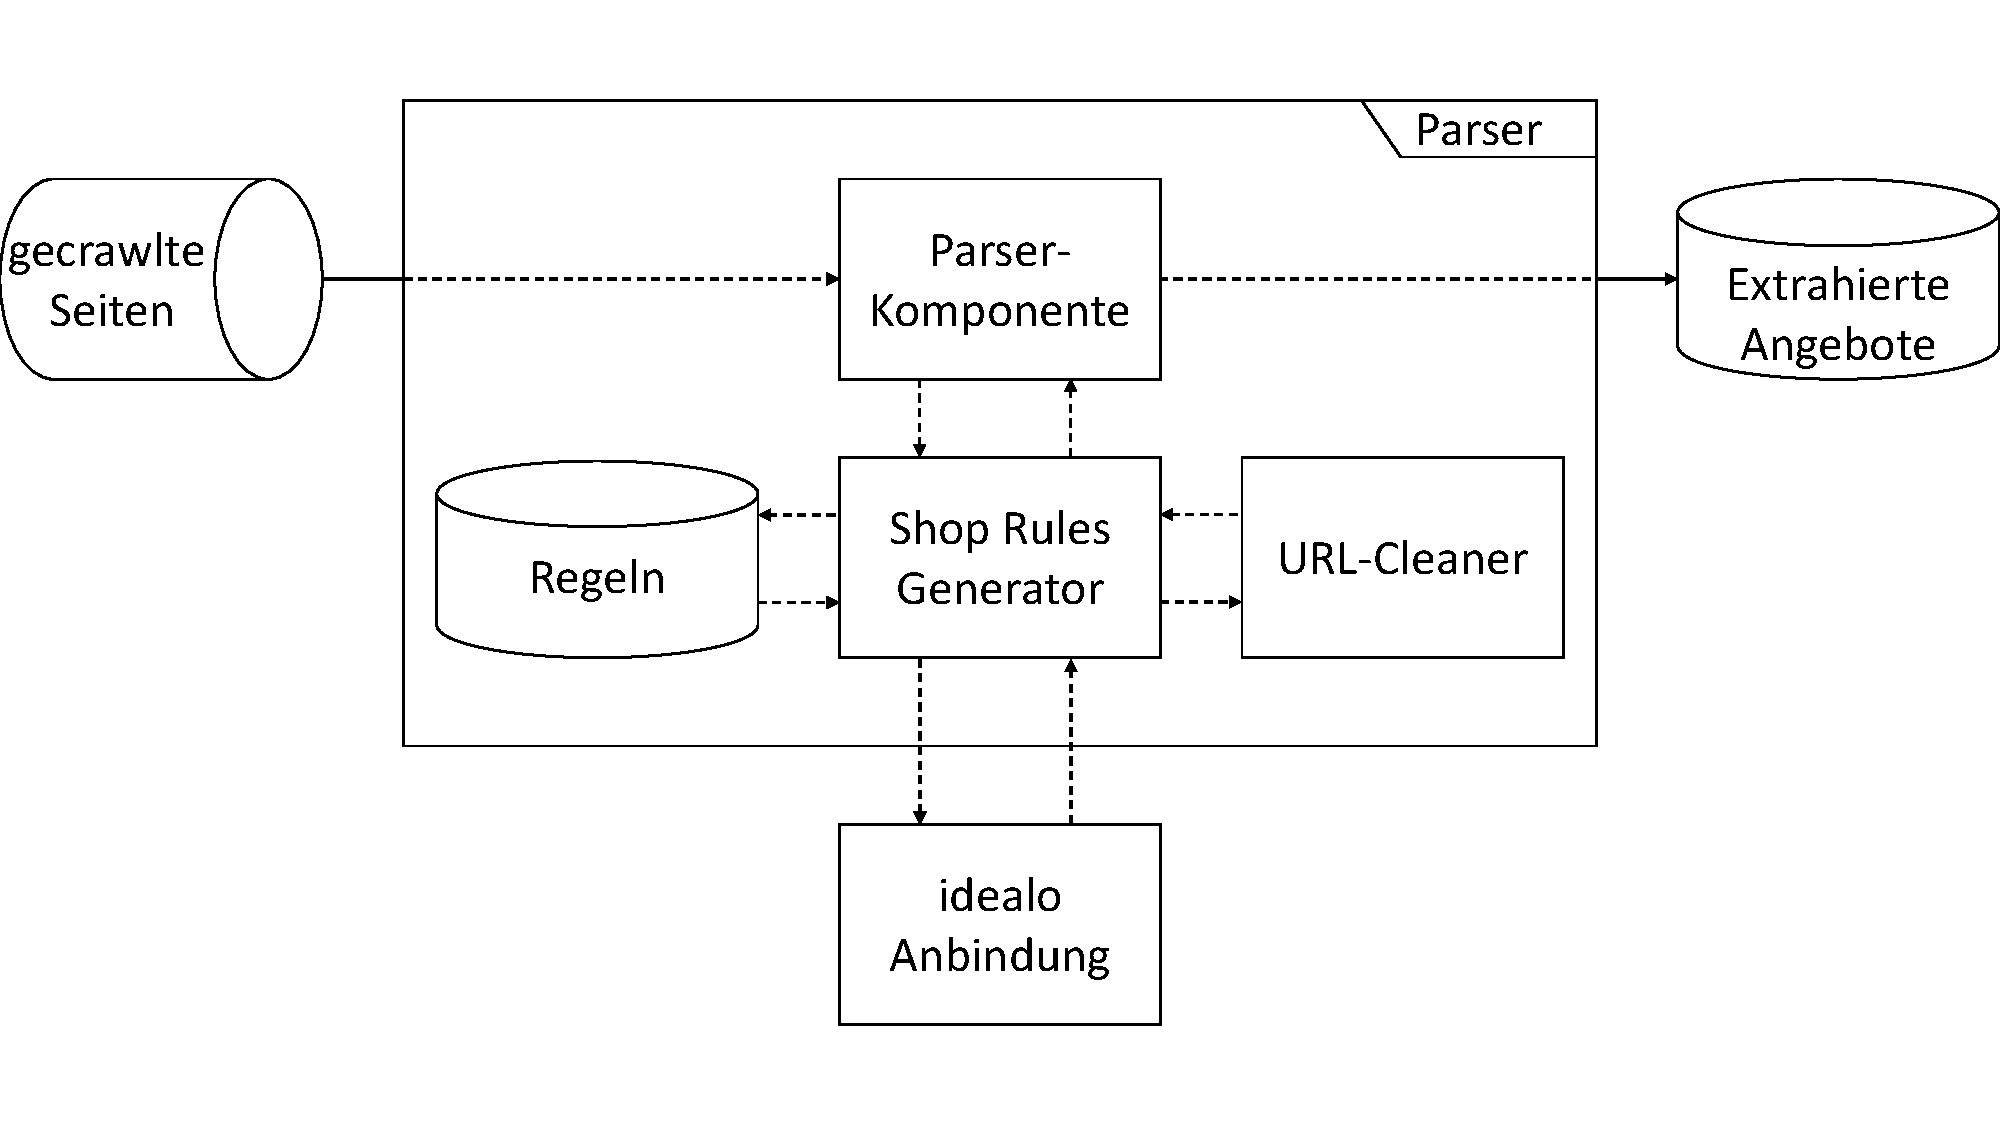
\includegraphics[width=\textwidth, trim=0 1.7cm 0 1.7cm, clip]{resources/Architektur-Parser.pdf}
    \caption{Architektur des Parsers}
    \label{abb:architektur-parser}
    \vspace{-0.5cm}
\end{figure}

Die \textit{Parser-Komponente} erhält ihre Eingaben, indem sie Nachrichten aus einer Queue konsumiert.
Eine Nachricht enthält eine vom Crawler heruntergeladene Webseite.
Der Crawler sendet zusätzlich zu jeder Seite, die Webadresse und die Identifikationsnummer des zugehörigen Shops mit.
Nach dem Erhalt einer Nachricht, lädt der Parser vom Shop Rules Generator (SRG) die Extraktionsregeln für den
entsprechenden Shop.

Sollten die Regeln noch nicht existieren, wartet der Parser solange, bis diese Regeln vom SRG erstellt wurden.
Sobald der Parser die Regeln empfangen hat, werden die Produktattribute aus der gecrawlten Seite extrahiert.
Zum Schluss werden die extrahierten Produktinformationen in einer Datenbank normalisiert abgespeichert.

Der Matcher greift später auf diese Datenbank für den Vergleich zu.
\\
~\\
Der \textit{Shop Rules Generator} gibt auf Anfrage die Regeln für einen beliebigen Shop zurück.
Sollten diese Regeln noch nicht existieren, werden sie generiert.
Während des Generierungsprozesses durchläuft der SRG mehrere Schritte.
In Abbildung~\ref{abb:datenfluss-srg} ist der Datenfluss des Vorgangs abgebildet.

\begin{figure}[H]
    \centering
    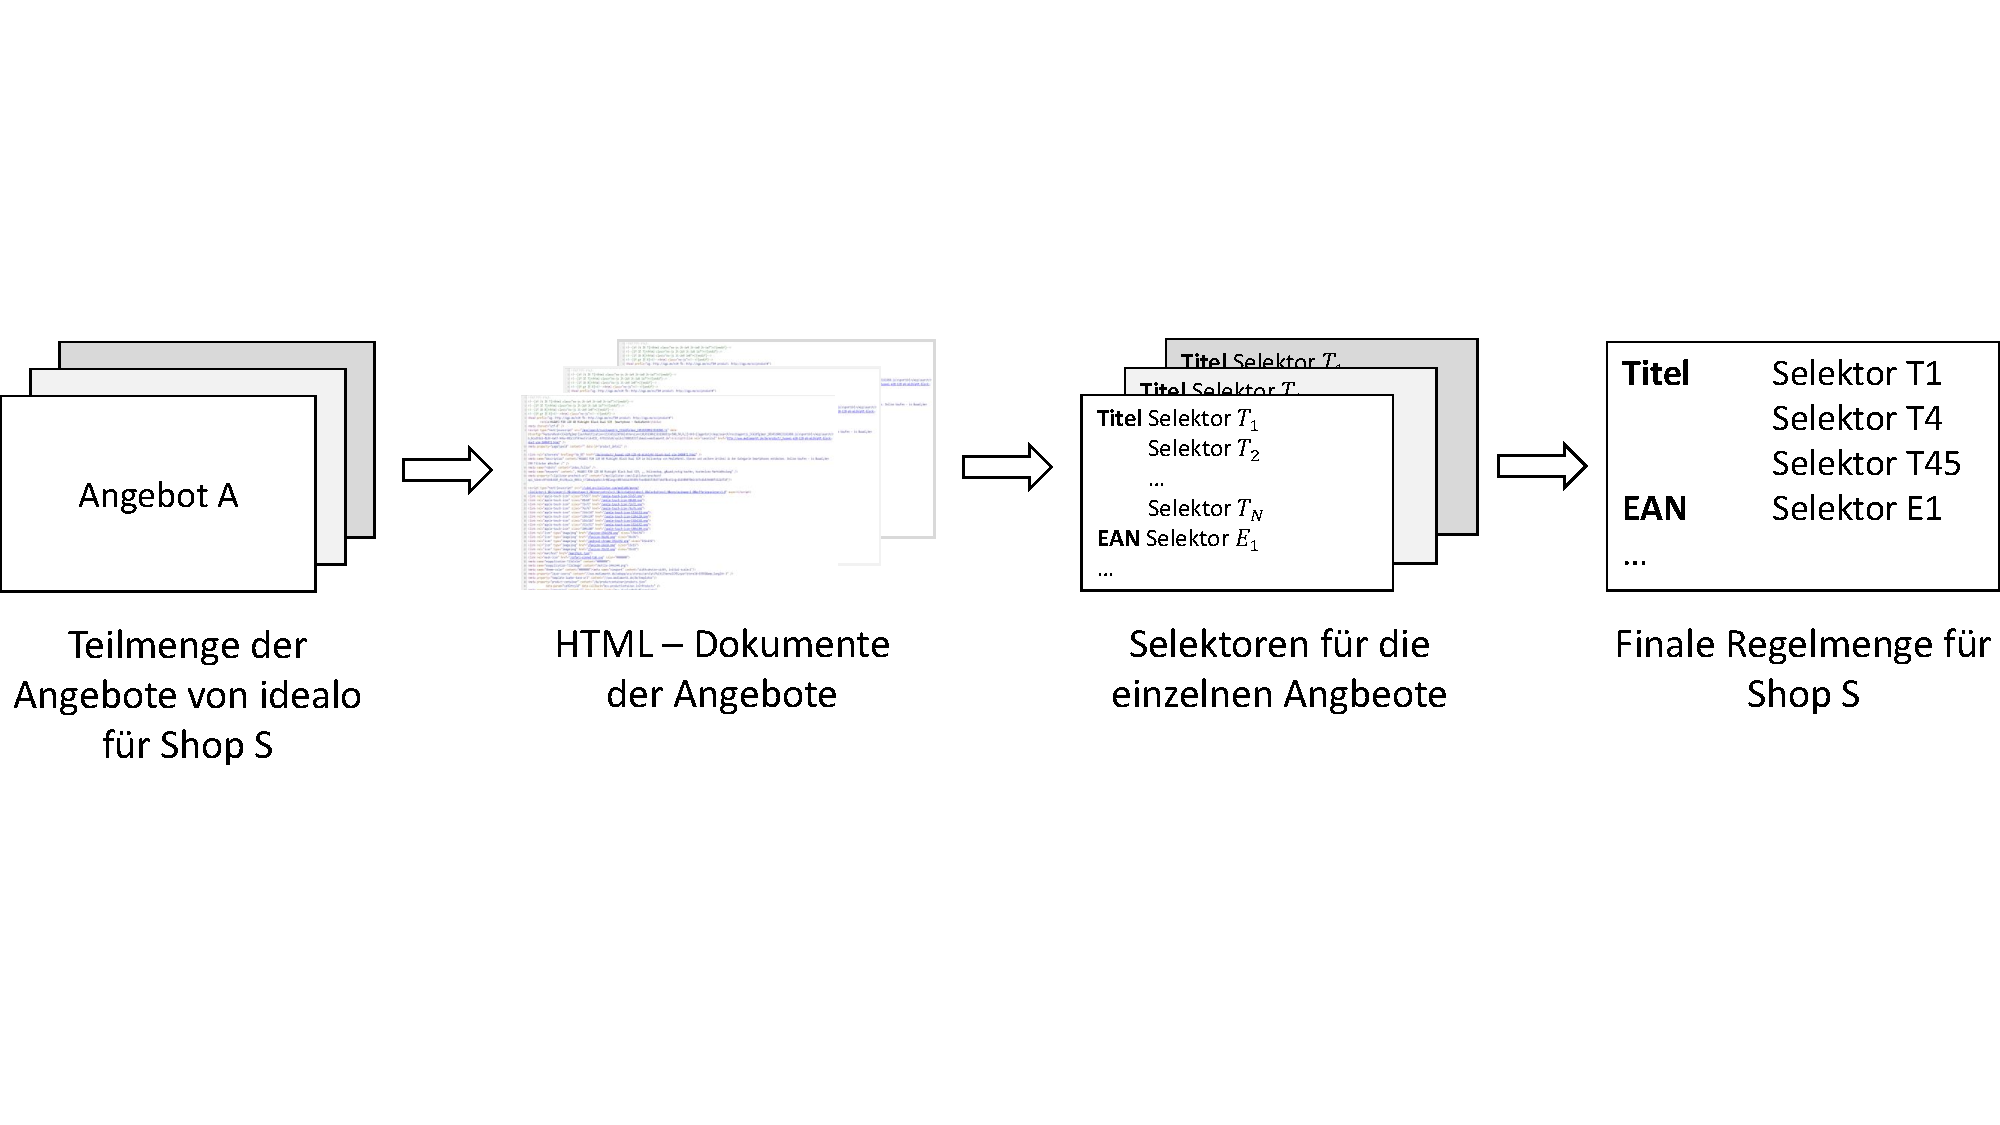
\includegraphics[width=\textwidth, trim=0 5cm 0 5cm, clip]{resources/Datenfluss-SRG.pdf}
    \caption{Datenfluss des Generierungsprozesses für einen Shop}
    \label{abb:datenfluss-srg}
    \vspace{-0.5cm}
\end{figure}

Zuerst wird eine bestimmte Anzahl von Angeboten aus der idealo-Datenbank geladen.
Die Anzahl der zu ladenden Angebote definieren wir als ``Sample Size'' und kürzen dieses mit $SaS$ ab.
Dieser Vorgang erfolgt über einen von idealo zur Verfügung gestellten API-Endpunkt, welcher den Datenbankzugriff über
eine REST-Schnittstelle kapselt.
Diese Vorgehensweise hat den Vorteil, dass wir die Infrastruktur von idealo nutzen können und keine Kopie der
Angebotsdaten lokal speichern müssen.

Zu jedem dieser Angebote liegen die Webadresse, sowie die Informationen über die in
Kapitel~\ref{subsec:technische-anforderungen-parser} genannten Produktattribute vor.
Außerdem wird für jedes Angebot das dazugehörige HTML-Dokument heruntergeladen.

Um die Server der Onlineshops nicht durch zu viele simultane Anfragen zu strapazieren, wird nach jedem
Download eine fest definierte Zeit gewartet.

Für die Menge der heruntergeladenen HTML-Dokumente ist somit bekannt, um welche Angebote es sich handelt und welche
konkreten Produktattribute erwartet werden.

Dieses Wissen wird für das Anlernen der Regeln genutzt.
Dazu werden die Werte aller Produkteigenschaften in dem HTML-Dokument gesucht.
Für jedes Vorkommnis eines Produktattributes wird ein Selektor erstellt, der den Fundort referenziert und einer Regel
zugeordnet.

Nachdem alle Regeln gesammelt wurden, werden diese bewertet.
Alle Regeln, die einem bestimmtem Qualitätsmaß entsprechen, werden in einer finale Regelmenge zusammengefasst und in
der Regeldatenbank für zukünftige Anfragen gespeichert.
\\
~\\
Einige Onlinehändler manipulieren vor der Übermittlung ihrer Angebote an idealo die Links zu deren Angeboten.
Sie fügen zu den regulären Webadressen Trackinginformationen hinzu.
Mit Hilfe dieser Trackinginformationen können sie nachvollziehen, welche Kunden durch idealo auf deren Seite gelandet
sind.

Diese Statistiken sind für die Shop-Besitzer wichtig, da sie somit die CPC-Abrechnung von idealo kontrollieren
können.
Die im Rahmen der Anlernphase getätigten Webseitenaufrufe könnten diese Tracking-Statistiken jedoch verfälschen.
Für idealo ist es deshalb wichtig, dass die Trackinginformationen vor dem Aufruf der Website entfernt werden.

Dazu haben wir die URL-Cleaner-Komponente entwickelt, welche Adressen mit Trackinginformationen als Eingabe erwartet und
bereinigt zurückgibt.

Der Fokus dieser Arbeit liegt auf der Funktionsweise des SRG.
Daher wird auf die konkrete Funktionsweise des URL-Cleaners nicht im Detail eingegangen.

\subsection{Die Erstellung der Selektoren}
\label{subsec:erstellen-von-selektoren}

Um einen Selektor zu erstellen muss zunächst ein konkretes Element der DOM-Hierarchie bestimmt werden.
Dieses Element wird von dem Shop Rules Generator (SRG) in einem vorherigen Schritt ermittelt und stellt den Fundort für
ein gewünschtes Produktattribut dar.
Es wird zwischen den folgenden drei Knotentypen unterschieden: Textknoten, Beschreibungsknoten und Datenknoten.
\textsc{Quelltext}~\ref{code:examples} enthält jeweils ein Beispiel für alle Knotentypen.
Der gesuchte Wert ist in diesem Fall die Produkteigenschaft EAN mit dem Produktattribut 9332721000108.

\vspace{0.25cm}
\lstset{
    escapeinside={(}{)},
    frame=lines,
    framerule=1pt,
    literate=%
    {Ö}{{\"O}}1
    {Ä}{{\"A}}1
    {Ü}{{\"U}}1
    {ß}{{\ss}}1
    {ü}{{\"u}}1
    {ä}{{\"a}}1
    {ö}{{\"o}}1,
    showstringspaces=false,
    xleftmargin=.25in,
    xrightmargin=.25in
}
\begin{minipage}[c]{\textwidth} % avoid page break within lstlisting
    \begin{lstlisting}[label={code:examples}]
<html>
    <head>
        <meta charset="utf-8">
        (\circled{2}) <meta itemprop='gtin13' content='9332721000108'>
        <script>(\ldots)<script>
        (\circled{3}) <script>
            function f() {
                var gtmGuaranteeProduct1 = {
                    "name":"Versicherung für 2 Jahre"
                };
                var product2400462 = {
                    "name":"Product",
                    "ean":"9332721000108"
                };
            }
        </script>
    </head>
    <body>
        <div id='product-details'>
            (\circled{1}) <span>9332721000108</span>
        </div>
    </body>
</html>
    \end{lstlisting}
    \vspace{-0.25cm}
    \captionof{lstlisting}{Beispiele für \circled{1} Textknoten, \circled{2} Beschreibungsknoten und \circled{3}
    Datenknoten}
    \vspace{0.25cm}
\end{minipage}

\textit{Textknoten} sind Elemente, bei denen das gewünschte Produktattribut innerhalb eines Tag-Paars steht.
Das Attribut ist somit ein sichtbarer Bestandteil der Browservisualisierung.

Zu den \textit{Beschreibungsknoten} gehören die Elemente, bei denen das gesuchte Produktattribut innerhalb der
Attributliste des Elementes vorkommt.
Dieses Attribut ist im Gegensatz zum Textknoten kein sichtbarer Bestandteil der Visualisierung.

Die Selektoren der beiden Knotentypen sind ähnlich aufgebaut und bestehen jeweils aus einem CSS-Selektor.
Der Aufbau des CSS-Selektors erfolgt analog zu der ``Copy~selector''-Funktion der Chrome-Entwicklertools.
Der Selektor für einen Beschreibungsknoten speichert zusätzlich einen Schlüssel, um das korrekte Elementattribut
auszulesen.
Die Selektoren für den Textknoten und den Beschreibungsknoten aus dem obigen Beispiel sind in
\textsc{Tabelle}~\ref{tab:textselektor-und-beschreibungsselektor} aufgeführt.
\begin{table}[h]
    \centering
    \begin{tabular}{ l | l | l}
        \textbf{Knotentyp}   &   \textbf{CSS-Selektor}    &   \textbf{Attribut} \\
        Textknoten  &   \#product-details > span:nth-of-type(1) & - \\
        Beschreibungsknoten &   html > head > meta:nth-of-type(1)[content]  & content
    \end{tabular}
        \caption{Selektoren für den \circled{1} Textknoten und \circled{2} Beschreibungsknoten}
    \label{tab:textselektor-und-beschreibungsselektor}
    \vspace{-0.5cm}
\end{table}
\\
~\\
Wir haben festgestellt, dass viele Internetshops Javascript auf ihrer Webseite verwenden.
Oftmals sind in diesem Fall die produktspezifischen Daten bereits in einer strukturierten Form im Javascript
als Objekt in der Javascript Objekt Notation (JSON) enthalten.
In dem gezeigten Beispiel im \textsc{Quelltext}~\ref{code:examples} ist ein solches Skript vereinfacht dargestellt.

Analog zum CSS-Selektor wollen wir nun das gleiche Prinzip auf das Javascript anwenden.

Der resultierende \textit{Datenselektor} wird aus drei Teilen gebildet.
Der erste Teil besteht, genau wie bei den anderen Selektortypen, aus einem \textit{CSS-Selektor}.
Dieser CSS-Selektor zeigt zu dem entsprechenden Script-Tag im DOM\@.

Um innerhalb des Javascriptes das richtige JSON-Objekt zu finden, wird ein Pfad verwendet, welcher durch die
verschiedenen Code-Blöcke navigiert.
Ein Block ist jeweils durch \textit{\{} und \textit{\}} markiert.
Der \textit{Block-Pfad} entsteht mit Hilfe einer Tiefensuche durch die verschachtelten Blöcke und zeigt auf einen
Block, welcher als JSON interpretiert werden kann.

Für die Navigation durch das JSON-Objekt wird ein \textit{JSONPath} erstellt.
Ein JSONPath ist ähnlich einem XPath aufgebaut ist somit standardisiert nutzbar.

Der resultierende Datenselektor sieht wie in \textsc{Tabelle}~\ref{tab:datenselektor} dargestellt aus.

\begin{table}[h]
    \centering
    \begin{tabular}{ l | l }
        \textbf{CSS-Selektor} &  html > head > script:nth-of-type(2)\\
        \textbf{Block-Pfad}   &  0 $\rightarrow$ 1\\
        \textbf{JsonPath}     &  \$['ean']
    \end{tabular}
    \caption{Selektor für den \circled{3} Datenknoten}
    \label{tab:datenselektor}
\end{table}

Häufig stehen vor und nach den gesuchten Produktattributen andere irrelevante Informationen.
Häufig befindet sich vor der gesuchten EAN zum Beispiel der String 'EAN:\textvisiblespace', welcher entfernt
werden sollte, um eine Bearbeitung überhaupt zu ermöglichen.
Eine generische Verbesserung, welche auf alle Selektoren angewendet werden kann, ist die Trimm-Funktion.

Diese Funktion fügt zu den generierten Selektoren Informationen hinzu, wie viele Stellen links oder rechts
abgeschnitten werden sollen.
Die Werte bezeichnen wir als Left-Cut und Right-Cut.

Sollte vor der gesuchten EAN immer derselbe String stehen, so gibt es keine Streuung in den Left-Cut-Werten.
Wenn es sich bei dem Produktattribut um die Beschreibung handelt und diese durch manuelle Änderungen von idealo von
denen der Webseite abweicht, so gibt es eine starke Streuung der Left- und Right-Cut-Werten.
\\
~~\\
Durch die verschiedenen Methoden Selektoren zu erstellen und durch die zuvor beschriebene Trim-Funktion wurde die
Flexibilität des Parser erhöht.
Dies hat jedoch den Nachteil das ein sogenanntes \textit{Rauschen} in den extrahierten Daten entsteht.

Dieses Rauschen entsteht dadurch, dass aus den gecrawlten HTML-Dokumenten viele Daten extrahiert werden,
bei denen nicht mehr bekannt ist, welche extrahierten Informationen korrekt oder falsch sind.
Damit die Anzahl der falsch extrahierten Produktattribute minimiert wird, haben wir ein Bewertungssystem für
Selektoren eingeführt.

Nach der Erstellung aller Selektoren, wird jedem Selektor ein Qualitätsindex zugewiesen.
Für jedes Angebot werden alle Selektoren angewandt und die extrahierten Produktattribute mit denen von idealo
verglichen.
Je nachdem ob der extrahierte Wert mit dem von idealo übereinstimmt, wird der Index erhöht oder verringert.

Ein Ausnahmefall bildet der leere String: Wird dieser String als extrahierter Wert zurückgegeben, so bleibt der
Qualitätsindex unverändert.
Wir haben uns für diese Variante entschieden, da man den leeren String von einem unerwünschten bzw.\
falschen Wert unterscheiden kann.

Bevor die Regeln mit dem Qualitätsindex in der Datenbank abgespeichert werden, werden diese auf das Intervall $[0; 1]$
normalisiert.
Alle Regeln mit einem normalisierten Index unter einem bestimmten Filterschwellwert $F$ werden verworfen.

Die Parser-Komponente verwendet den Qualitätsindex, um aus allen gefundenen Werten den Besten zu ermitteln.
Dazu gruppiert sie nach den extrahierten Werten und summiert den normalisierten Index.
Für jedes Produktattribut wird somit nur das beste Ergebnis gespeichert.